\documentclass{standalone}
\usepackage{tikz}
\usepackage{tkz-graph}
\usepackage{tkz-berge}

\begin{document}

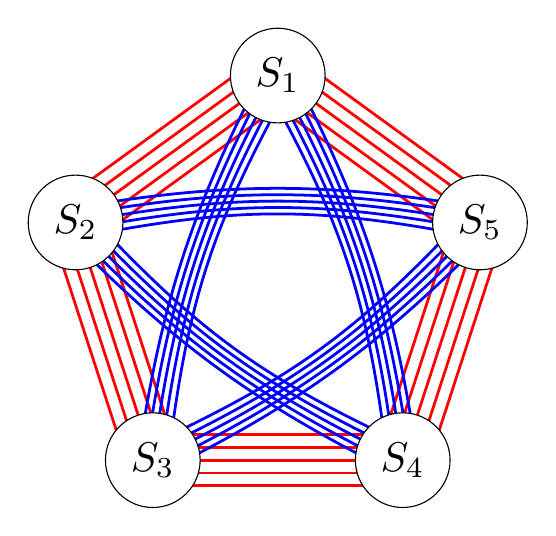
\begin{tikzpicture}
\GraphInit[vstyle=Hasse]
\tikzset{VertexStyle/.style = {shape = circle,fill = white,inner sep = 0pt,outer sep = 0pt,minimum size = 8pt,draw}}

{\tikzset{EdgeStyle/.append style = {red,line width=1.0pt}}
  \grCycle[RA=(3.0-0.7),prefix=a,rotation= 90]{5};
  \grCycle[RA=(3.2-0.7),prefix=a,rotation= 90]{5};
  \grCycle[RA=(3.4-0.7),prefix=a,rotation= 90]{5};
  \grCycle[RA=(3.6-0.7),prefix=a,rotation= 90]{5};
  \grCycle[RA=(3.8-0.7),prefix=a,rotation= 90]{5};
}

{\tikzset{EdgeStyle/.append style = {blue,line width=1.0pt}}
  \tikzset{EdgeStyle/.append style = {bend left=10}}
  \grEmptyCycle[RA=(3.0-0.7),prefix=a,rotation= 90]{5};
  \EdgeInGraphMod{a}{5}{2};
  \grEmptyCycle[RA=(3.2-0.7),prefix=a,rotation= 90]{5};
  \EdgeInGraphMod{a}{5}{2};
  \grEmptyCycle[RA=(3.4-0.7),prefix=a,rotation= 90]{5};
  \EdgeInGraphMod{a}{5}{2};
  \grEmptyCycle[RA=(3.6-0.7),prefix=a,rotation= 90]{5};
  \EdgeInGraphMod{a}{5}{2};
  \grEmptyCycle[RA=(3.8-0.7),prefix=a,rotation= 90]{5};
  \EdgeInGraphMod{a}{5}{2};
}
\grEmptyCycle[RA=(3.4-0.7),prefix=a,rotation= 90]{5};

\tikzstyle{region}=[circle, draw=black, fill=white, minimum size=20pt, fill=white, scale=1.5];
\node[region] at (a0) {$S_1$};
\node[region] at (a1) {$S_2$};
\node[region] at (a2) {$S_3$};
\node[region] at (a3) {$S_4$};
\node[region] at (a4) {$S_5$};

\end{tikzpicture}

\end{document}
